\documentclass[10pt]{article}

% %%%%%%%%%%%%%%%%%%%%%%%%%%%%%%%%%%%%%%%%%%%%%%%%%%%%%%%%%%%%%%%%%%%%%%%%%%%%%%
% %                                 PACKAGES                                   %
% %%%%%%%%%%%%%%%%%%%%%%%%%%%%%%%%%%%%%%%%%%%%%%%%%%%%%%%%%%%%%%%%%%%%%%%%%%%%%%
% Identifies input coming with an UTF-8 format
\usepackage[utf8]{inputenc}
% Uses 8-bit T1 fonts (Latin) 
\usepackage{setspace}
 \singlespacing
% Arial font.
\usepackage[scaled]{helvet}
\renewcommand\familydefault{\sfdefault}
\usepackage[T1]{fontenc}
\setlength{\parindent}{0.4cm}
% Equations
\usepackage{amsmath}
% Enum Item
\usepackage{enumitem}
% Easy Lists
\usepackage[ampersand]{easylist}
% Tables
\usepackage{booktabs}
\usepackage{longtable}
% Hyperreferences
\usepackage{hyperref}
% Images
\usepackage{graphicx}
% Set images location
\usepackage{wrapfig}
% Position for tables and images
\usepackage{float}
% Blibliography
\usepackage[backend=biber, style=numeric]{biblatex}
 \addbibresource{paper.bib}

\begin{document}

\title{PL3 - Cloud Computing}

\author{Pablo Acereda \and
David E. Craciunescu \and
Ángel Martín \and
Ángelo Moreno \and
Laura Pérez
}

\institute{Universidad de Alcalá de Henares - EPS}

\maketitle

\section{Contenedores}

\section{IA \& Machine Learning}

\section{IoT}

\section{Seguridad}

\section{Web \& Logic Apps}

La parte de Web \& Logic Apps tiene un amplio espectro de trabajo, podemos realizar
múltiples aplicaciones y servicios que aporten una perspectiva interesante y que
permitan interactuar con ellas a un nivel satisfactorio.

De entre todas ellas, se ha elegido realizar una aplicación web con conexión remota.
Será implementada tanto en Microsoft Azure como en Amazon Web Services, y
posteriormente evaluada en función de la plataforma.

\subsection{Prerrequisitos}

Para realizar todo esto, primero se debe disponer de ciertas aplicaciones y
recursos. Comenzando con la creación de las máquinas virtuales (en este caso con
distribución Linux) sobre las que se va a desarrollar la aplicación, tanto en Azure
como en AWS.

En Azure, la creación de la máquina virtual será similar a la desarrollada en la
parte obligatoria, pero se van a añadir unos requisitos que serán necesarios
posteriormente. Estos son: creación de una IP estática y abrir los puertos 3000 y
5000. La IP estática será necesaria para mantener un contacto directo entre el
servidor y la aplicación, y evitar cambiar continuadamente la IP, con los problemas
que puede acarrear. Abrir los puertos 3000 y 5000 se lleva a cabo para que la
comunicación esté identificada en todo momento y se sepa a qué puerto llevar la
información.

\begin{figure}[h!]
 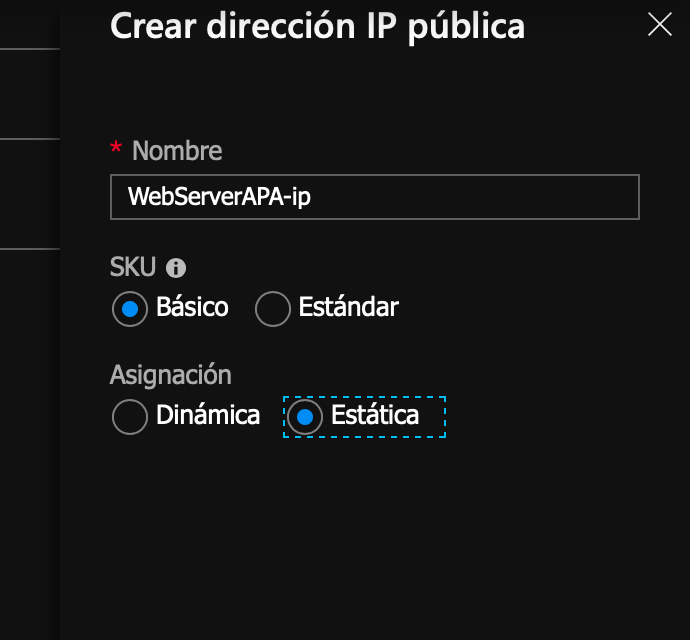
\includegraphics[width=\linewidth]{./Web/Azure/Azure1.png}
 \caption{Selección de IP estática.}
\end{figure}

\begin{figure}[h!]
 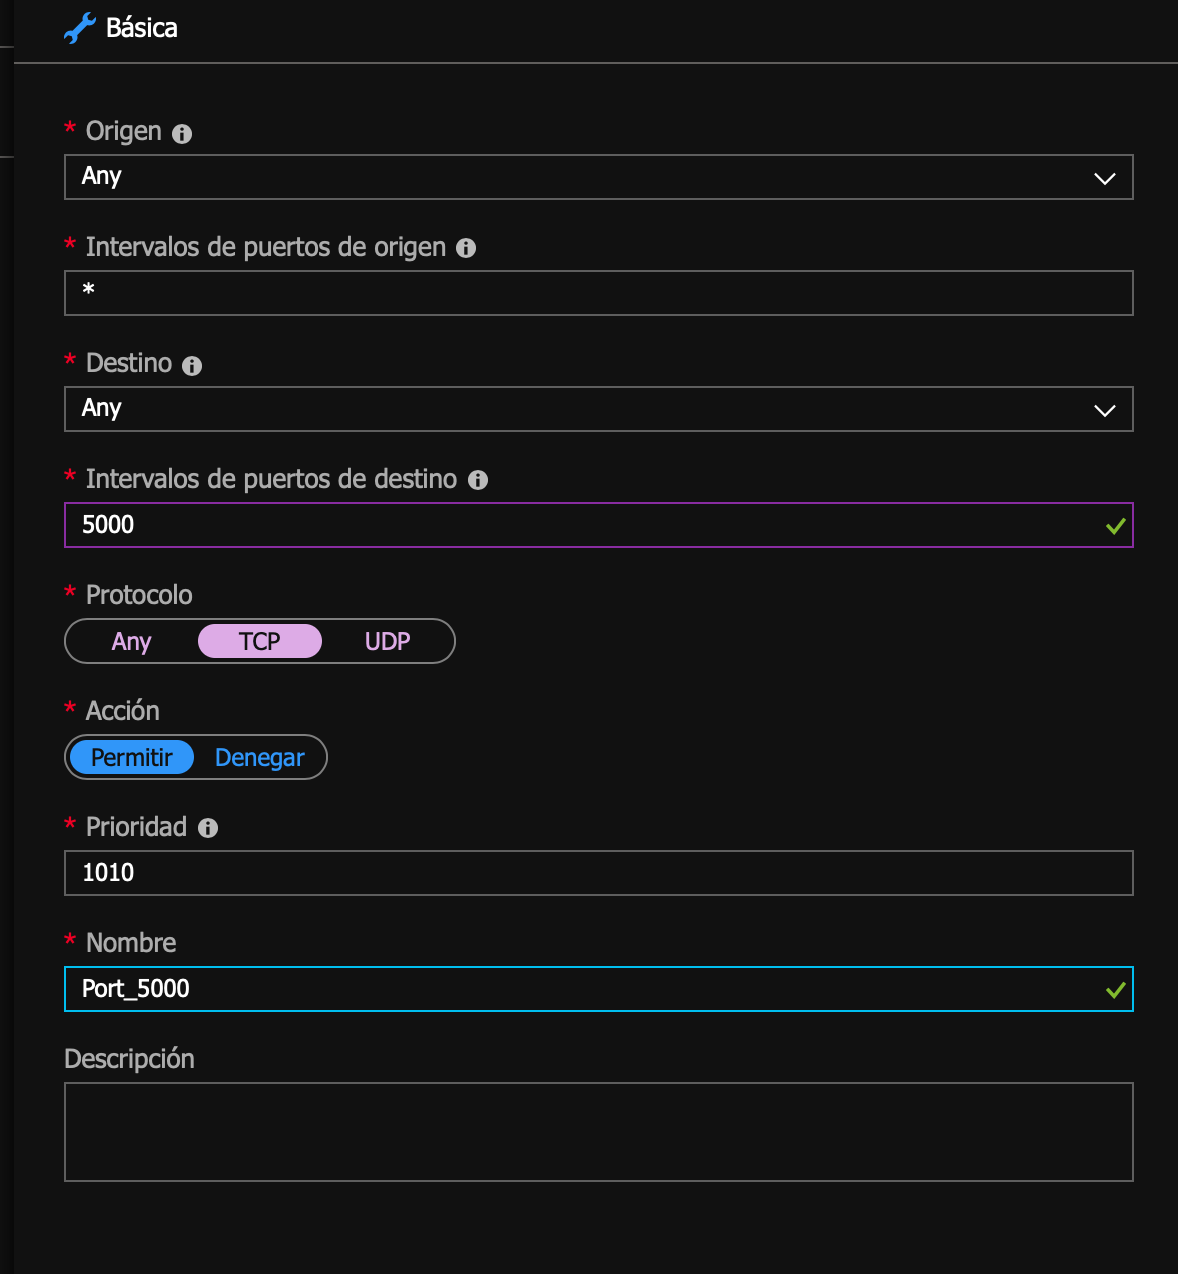
\includegraphics[width=\linewidth]{./Web/Azure/Azure2.png}
 \caption{Abrir puerto 5000.}
\end{figure}

\begin{figure}[h!]
 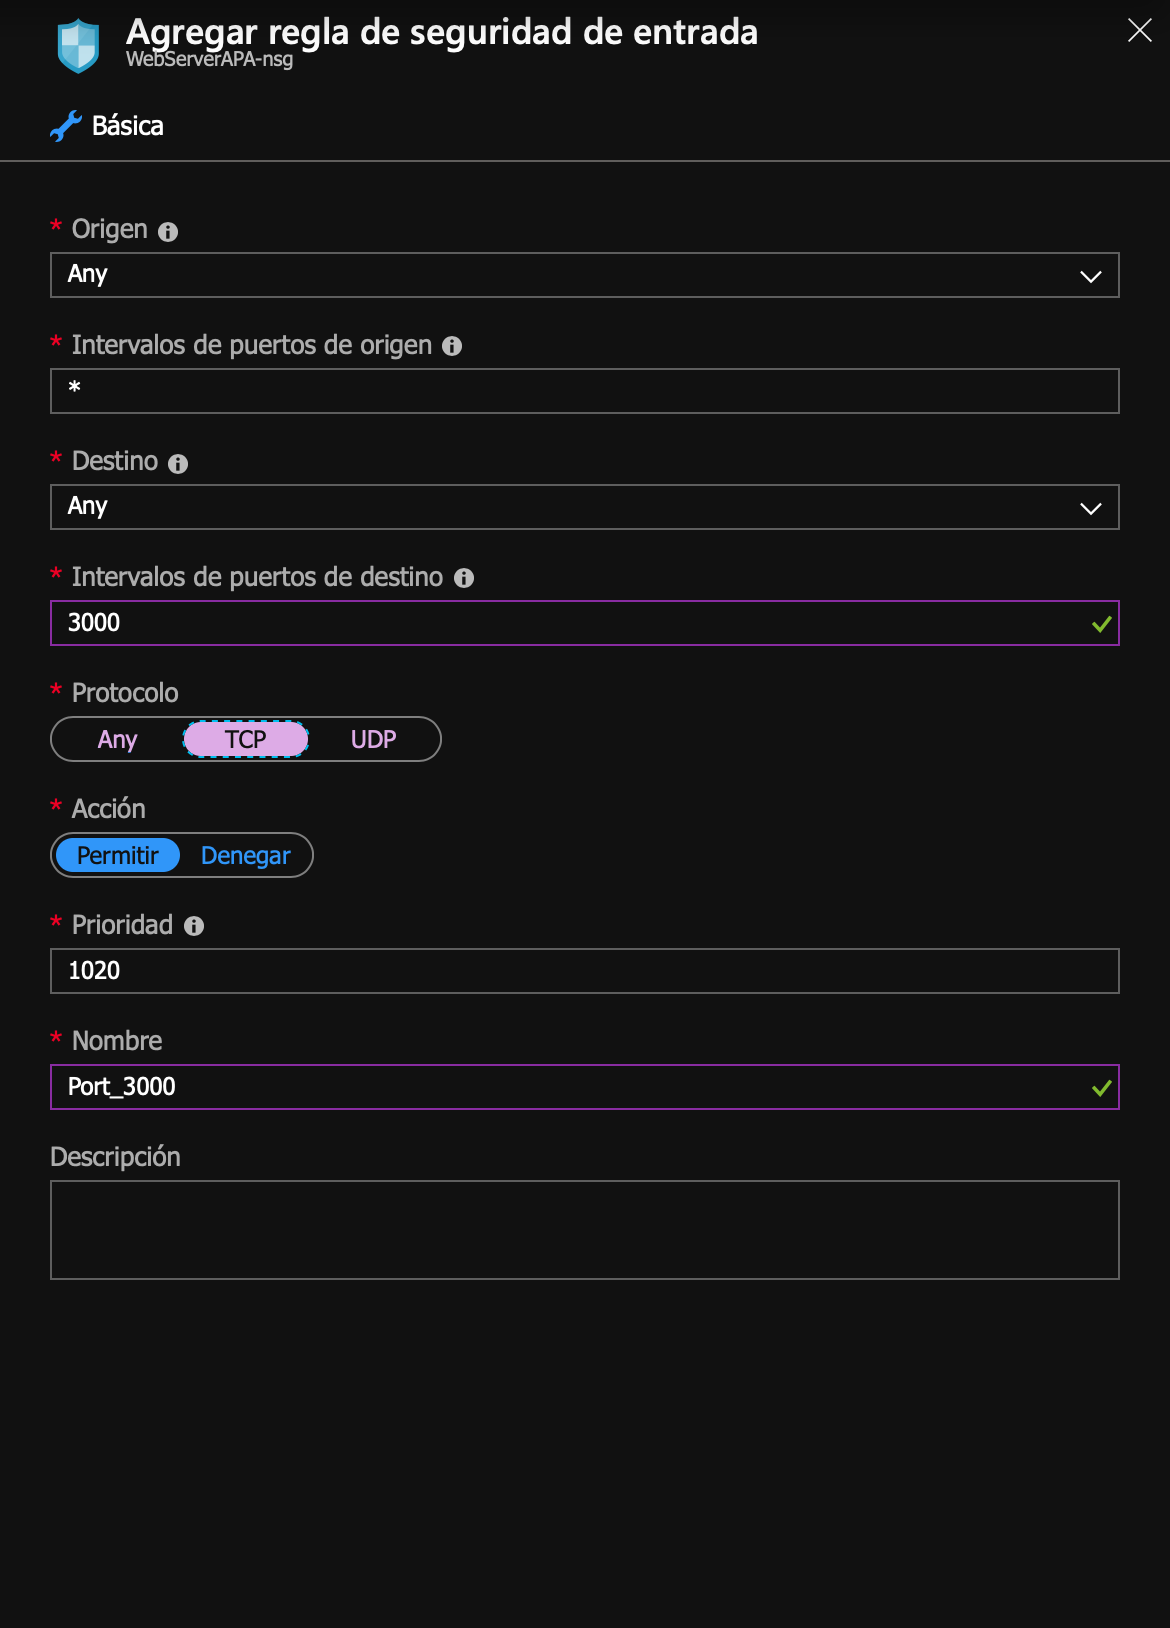
\includegraphics[width=\linewidth]{./Web/Azure/Azure3.png}
 \caption{Abrir puerto 3000.}
\end{figure}

Tras esto, se realizará lo mismo en AWS, pero con las variaciones que la plataforma
requiere. Primero, hay que crear la instancia de Linux que se va a utilizar. En
este caso se utilizarán las características mínimas para no consumir demasiados
recursos.

\begin{figure}[h!]
 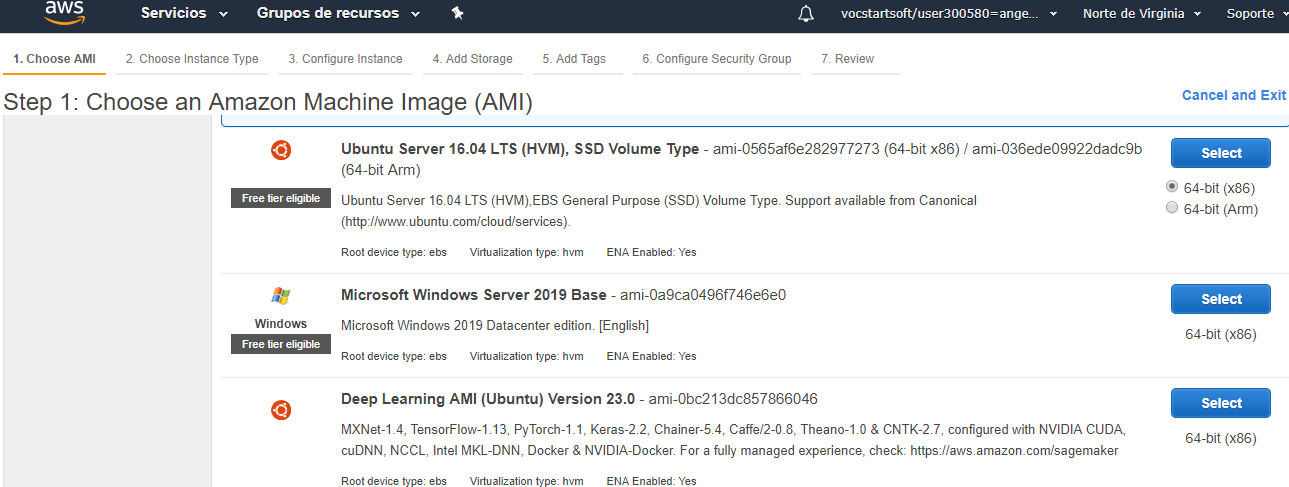
\includegraphics[width=\linewidth]{./Web/AWS/AWS1.png}
 \caption{Selección de MV.}
\end{figure}

\begin{figure}[h!]
 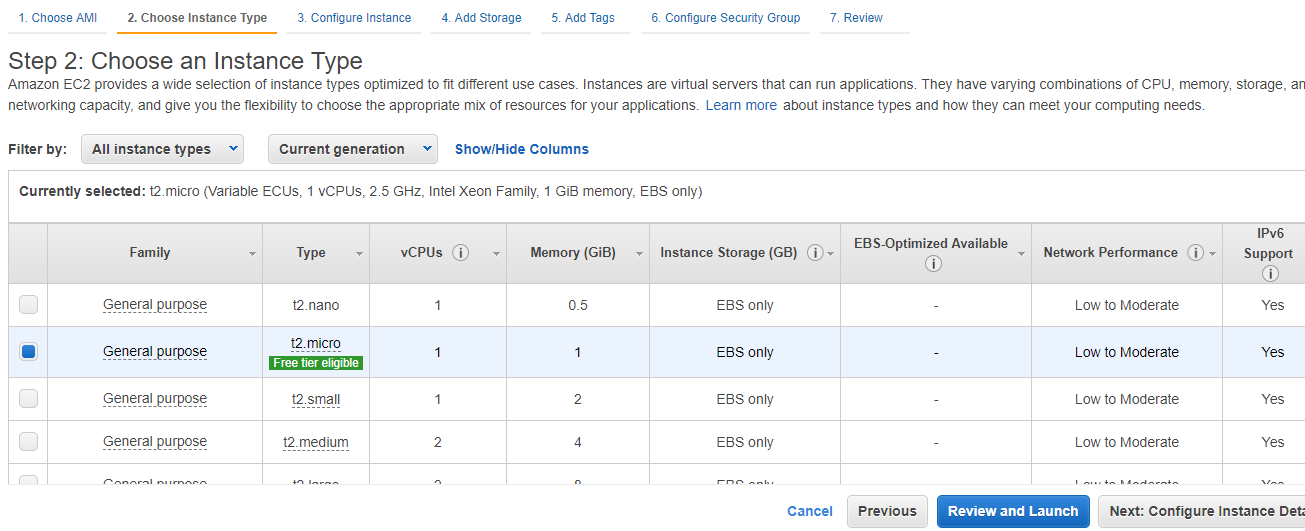
\includegraphics[width=\linewidth]{./Web/AWS/AWS2.png}
 \caption{Elección de características.}
\end{figure}

Después, al igual que con Azure, se abrirán los puertos 3000 y 5000, por lo
explicado anteriormente; y se crea una IP elástica, que te proporciona el propio
AWS.

\begin{figure}[h!]
 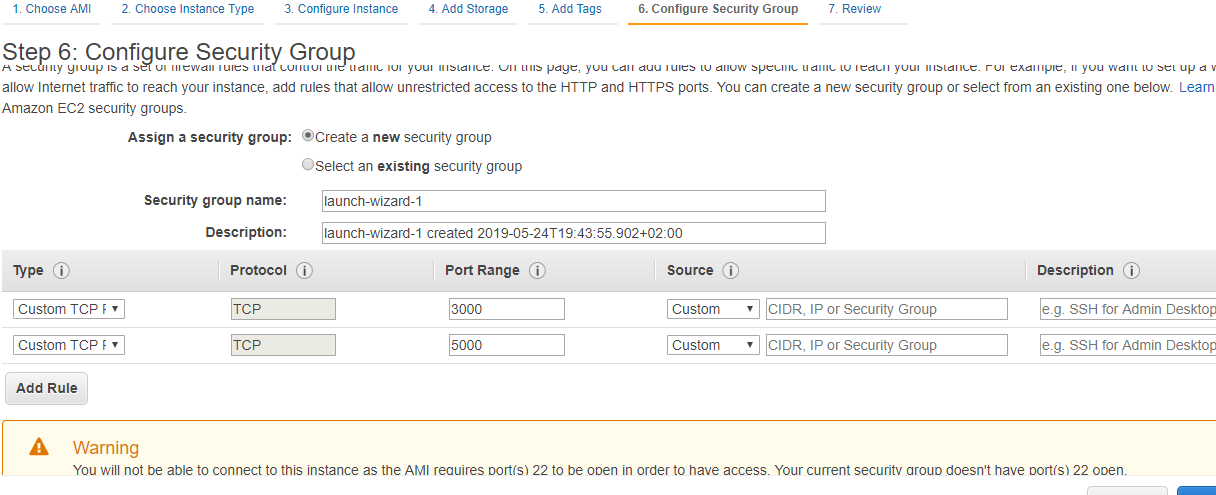
\includegraphics[width=\linewidth]{./Web/AWS/AWS3.png}
 \caption{Abrir puertos.}
\end{figure}

Una vez realizado esto, la plataforma pide que se descarguen un par de claves
privadas para la conexión con la instancia, por lo tanto, se descarga el archivo
con las claves y se ubica en algún directorio que se pueda recordar fácilmente,
dado que más tarde será necesario.

Cuando se tienen listas ambas máquinas virtuales, hay que realizar la conexión ssh
mediante la terminal para conectarse a ellas. En Azure, mediante el usuario, la IP
estática y la contraseña, y en AWS mediante el usuario, la IP estática y la ruta
donde se ha ubicado el archivo con las claves privadas.

Ya dentro de las máquinas virtuales, se instalarán Python 3, NodeJS y npm, tanto en
la de Azure como en la de AWS.

\subsection{Funcionamiento}

Para el desarrollo y la implementación de la aplicación, se comenzará con la
creación del código necesario para ella. En este caso, se ha recurrido tanto a
Python 3 como a React, dadas las amplias opciones que nos proporcionan y lo
sencillo que resulta desarrollar cualquier cosa con estos lenguajes. El código se
expone a continuación:

\begin{figure}[h!]
 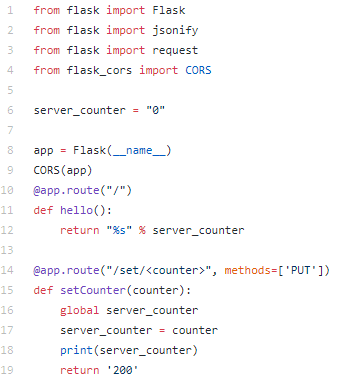
\includegraphics[width=\linewidth]{./Web/Azure/CodigoServer.png}
 \caption{Código para el Servidor.}
\end{figure}

\begin{figure}[h!]
 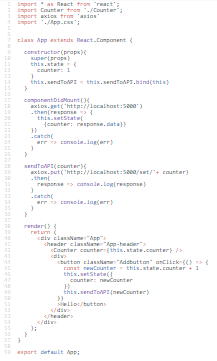
\includegraphics[width=\linewidth]{./Web/Azure/CodigoWeb1.png}
 \caption{Código para la Web.}
\end{figure}

En sí, lo que se está realizando es una página web con un texto, un contador y un
botón. El botón será para ir incrementando el contador de forma remota y que sea
registrado.

Para comprobar el funcionamiento de la aplicación, se abren dos terminales para la
plataforma sobre la que vayamos a trabajar, se lleva a cabo la conexión ssh con lo
mencionado anteriormente y, dado que el código ha sido alojado en repositorios de
Git, se clonan ambos repositorios en el directorio de trabajo que se desee. Una vez
hecho, dentro del repositorio donde está la parte de la web, se ejecuta el comando
“npm start”, para iniciar la conexión de la página web. Como los pasos a seguir son
los mismos en ambas plataformas, se va a mostrar lo de una de ellas (aplicable a la
otra por igual).

\begin{figure}[h!]
 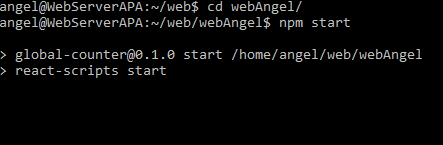
\includegraphics[width=\linewidth]{./Web/Azure/ConexionWeb.png}
 \caption{Conexión de la web.}
\end{figure}

Mientras, en la otra terminal, para iniciar el servidor llamamos al comando "FLASK APP=main.py flask run –host=0.0.0.0".

\begin{figure}[h!]
 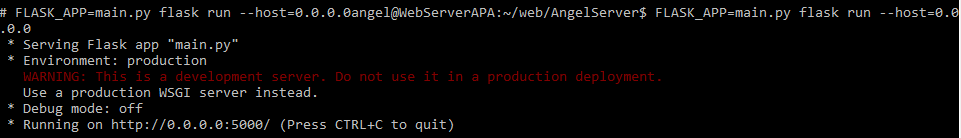
\includegraphics[width=\linewidth]{./Web/Azure/ConexionServer.png}
 \caption{Conexión del Servidor.}
\end{figure}

Con esto se tiene tanto la web activa, como el servidor para realizar los cambios
iniciado. Para comprobarlo se accede a la url de la web “ip-estática:3000”, y se
pulsa varias veces el botón del contador.

\begin{figure}[h!]
 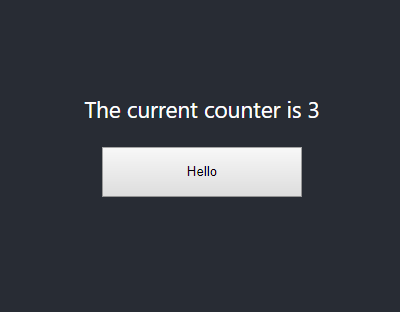
\includegraphics[width=\linewidth]{./Web/Azure/Contador.png}
 \caption{Contador en la web.}
\end{figure}

Se puede observar que el contador aumenta, y si se comprueba la terminal en la que
se ha iniciado el servidor, aparecen las peticiones que ha recibido y el estado en
cada momento de dicho contador.

\begin{figure}[h!]
 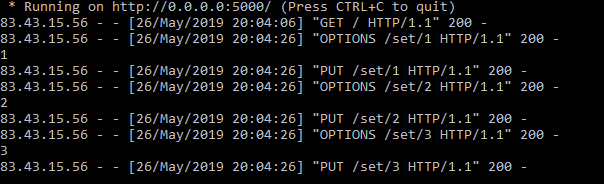
\includegraphics[width=\linewidth]{./Web/Azure/Comprobacion.png}
 \caption{Comprobación en el Servidor.}
\end{figure}

\subsection{Comparación}

Por útlimo, como comparación entre ambas plataformas, a la hora de crear e iniciar
los recursos, Azure ofrece más facilidades y más variedad que AWS. Azure tiene
mucha más variedad de entornos y utilidades para empezar a desarrollar, mientras
que AWS lo tiene más limitado y el acceso está restringido a algunos de los
recursos (por lo menos para la cuenta de estudiantes). Pero también hay que
destacar que AWS ofrece unos protocolos de seguridad más extrictos y a la hora de
iniciar las conexiones y utilizar los recursos es más veloz que Azure.

Por lo tanto, si se quiere utilizar en un ámbito menos profesional y sin llevar a
cabo grandes proyectos, se recomienda el uso de Microsoft Azure. Pero si se
pretende hacer un proyecto empresarial a mayor escala, y se disponen de los
recursos y el personal adecuados, se recomienda la utilización de Amazon Web
Services.

\end{document}

